\section{Datenvisualisierung}
\label{sec:Datenvisualiserung}
Ein weiteres Ziel der Studienarbeit war es die gesammelten Daten zu präsentieren. Die Entscheidung fiel auf eine Webapplikation. Der Grund für diese Entscheidung war, dass die Anwendung von vielen verschiedenen Geräten genutzt werden kann. Die Webseite kann unter \textit{ http://sensorknoteniot.it.dh-karlsruhe.de/} aufgerufen werden, der Benutzername lautet \textit{tester} mit dem Kennwort \textit{python}.

Als Technologie wurde AngularJS gewählt, ein clientseitiges JavaScript Webframework zur Erstellung von Singel-Page-Webanwendungen. Zur Präsentation der Webseite wurde HTML5 und CSS3 eingesetzt. Zur Oberflächengestaltung wurde Bootstrap (CSS-Framework) eingesetzt.

Die Webseite besteht aus drei Seiten insgesamt. Auf diese kann erst nach einer Authentifizierung zugegriffen werden. Die Webseite nutzt den in Kapitel \ref{sec:webservice} vorgestellten REST Webservice, um auf die Daten aus der Datenbank zuzugreifen.
\begin{figure}
	\centering
	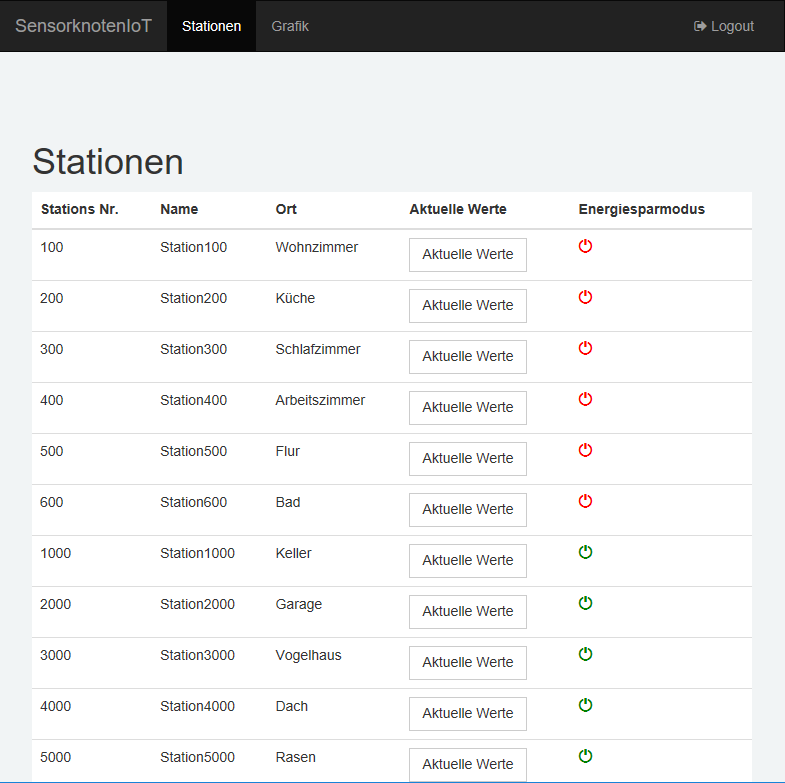
\includegraphics[width=0.6\textwidth]{bilder/WebseiteUebersicht}
	\caption{Webseite: Übersicht aller Sensorknoten}
	\label{img:WebseiteUebersicht}
\end{figure}

\paragraph{Übersicht aller Sensorknoten} Zunächst erhält der Nutzer, wie in Bild \ref{WebseiteUebersicht}, eine Übersicht über alle Sensorknoten. Die Übersicht enthält dabei alle Sensorknoten, die bereits einmal einen Datensatz in der Datenbank gespeichert haben.

Die Daten werden in einer Tabelle dargestellt. Diese enthält dabei Informationen zur Stations Nummer, Name der Station, der Ort an dem sich das Gerät befindet und ob die Station sich im Energiesparmodus befindet oder nicht. Von dieser Übersichtsseite gelangt der Nutzer mit dem Button \textit{Aktuelle Werte} zu den aktuellen Werten des Sensorknotens. 
\begin{figure}
	\centering
	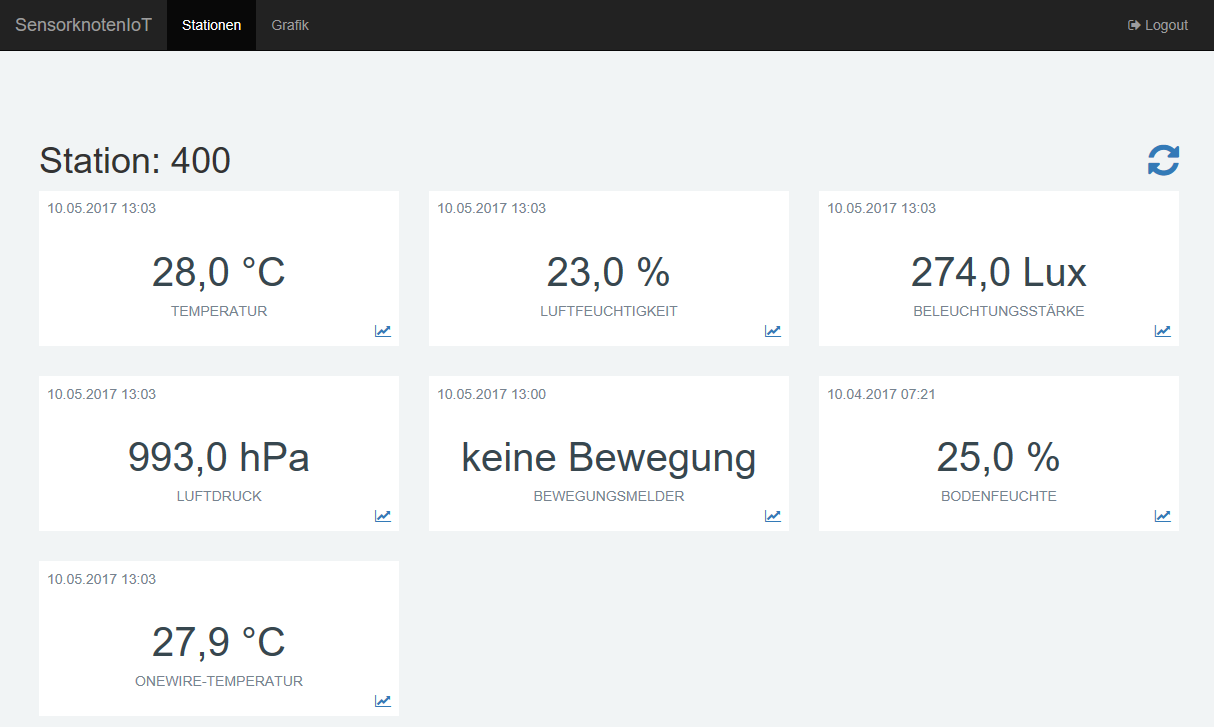
\includegraphics[width=0.7\textwidth]{bilder/WebseiteSensorknotenAktuell}
	\caption{Webseite: Aktuelle Übersicht eines Sensorknotens}
	\label{img:WebseiteSensorknotenAktuell}
\end{figure}
\paragraph{Aktuelle Werte eines Sensorknotens} Auf dieser Seite kann sich der Nutzer die aktuellsten Werte des Sensorknotens anzeigen lassen. Die Anzahl der Kacheln wird dynamisch erzeugt, dies hängt davon ab,  welche Messwerte der Sensorknoten bereits gesendet hat. In einer Kachel sind die Informationen enthalten, wann der Messwert gemessen wurde, welchen Wert der Messwert hat und welche Einheit dieser hat. Zusätzlich ist noch ein Button auf jeder Kachel bei dem sich der Nutzer zusätzlich die Grafik der vergangene Werte anzeigen lassen kann. Die Webseite aktualisiert die Daten alle 30 Sekunden. Es besteht aber auch die Möglichkeit(Button oben rechts) eine manuelle Aktualisierung anzustoßen.
\begin{figure}
	\centering
	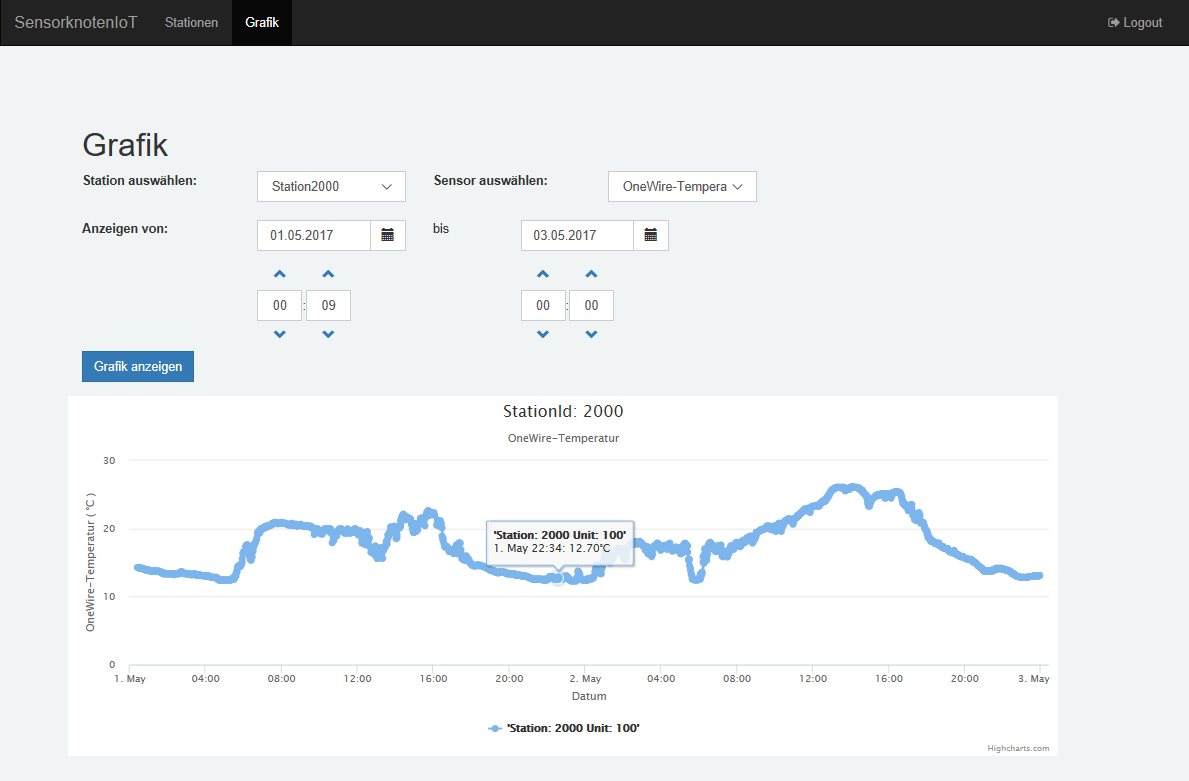
\includegraphics[width=0.7\textwidth]{bilder/WebseiteGrafik}
	\caption{Webseite: Grafik eines Messwertedatensatz}
	\label{img:WebseiteGrafik}
\end{figure}

\paragraph{Grafik über einen bestimmten Zeitraum} Zur Ansicht älterer Sensorwerte besteht die Möglichkeit sich die gesammelten Werte in einem Kurvendiagramm darzustellen. Der Nutzer muss zunächst die Station und den Sensorwert auswählen den er betrachten möchte. Anschließend muss er angeben in welchem Zeitraum er die Messwerte dargestellt haben möchte. Mit dem Betätigen des „Buttons Grafik anzeigen“ wird die Grafik angezeigt. In der x-Achse befindet sich das Datum, in der y-Achse ausgewählte Wert. Die x- und y-Achse wird entsprechend der gewählten Größen angepasst. Mit der Maus kann über die Kurve gefahren werden und sich mit Hilfe eines Tooltipps genauere Informationen anzeigen zu lassen. Für die Grafikanzeige wurde ein JavaScript Plugin verwendet mit dem verschiedene Diagrammtypen dargestellt werden können. Als Framework wurde \textit{Highcharts} verwendet. Momentan werden noch alle Werte angezeigt. Hier könnte bei einer großen Anzahl an Messwerten eine Reduzierung / Ausdünnung vorgenommen werden.
